% Files using this must be two subfolders
% deep. Adjust the number of ../ for the
% depth of the file.
% Imports
\usepackage{fancyhdr}
\usepackage{geometry}
\usepackage{icomma}
\usepackage{amsmath}
\usepackage{multicol}
\usepackage{mathptmx}
\usepackage{anyfontsize}
\usepackage{t1enc}
\usepackage{tabto}
\usepackage{listings}
\usepackage{filecontents}
\usepackage{subcaption}
\usepackage{tikz}
\usepackage[parfill]{parskip}
\usepackage{graphicx}
\usepackage[]{mdframed}
\usepackage{amsmath}
\usepackage[makeroom]{cancel}
\usepackage{pgfplots}
\usepackage{pgfplotstable}
\usepackage{xfrac}
\usepackage{amssymb}
\usepackage{mathtools}
\pgfplotsset{compat=1.18}
\usetikzlibrary{patterns}
\usepgfplotslibrary{polar}
\usepgfplotslibrary{fillbetween}

\geometry{margin=2.5cm}

\newcommand{\name}{Kaleb Burris}
\newcommand{\classname}{MATH F253, Elizabeth S. Allman, University of Alaska Fairbanks}
\newcommand{\assignment}{FILL IN ASSIGNMENT NAME}

\pagestyle{fancy}

\fancyhead[L]{
    \name 
    \newline
    \classname
    \newline
    \assignment
}

\newcommand{\horizontal}{\noindent\rule{\hsize}{0.4pt}}

\setlength{\headheight}{42pt}
\setlength{\headsep}{0.25in}
\setlength{\columnsep}{0.35cm}
\setlength{\columnseprule}{1pt}

\usepackage[T1]{fontenc}
\usepackage{lmodern}
\usepackage{tkz-fct}

% Put class number, class name, and professor 
% name.
% Use only in case of emergency, this
% should be covered by the preamble.
% \renewcommand\classname{}

% Put the assignment name with \S if 
% necessary for the section and the question 
% numbers.
\renewcommand\assignment{Final Review}

\begin{document}
    % Templates
    \iffalse
    % Use these for equations.
    \begin{equation*}
        \begin{gathered}
            Equations go here.
        \end{gathered}
    \end{equation*}

    % Use this if a line of math is too long.
    \resizebox{\hsize}{!}{$Long equation goes here$}

    % Use these for multiple columns.
    \begin{multicol*}{# of columns}
        % Remove the * if you want the columns to be balanced.
    \end{multicol*}

    % Use this to add a horizontal line.
    \horizontal

    \fi

    % Begin homework here.
    %%%%%%%%%%%%%%%%%%%%%%

    \section*{Part I}

    \begin{itemize}
        \item [1.] Evaluate $\int_{1}^{\infty} \frac{1}{1+x^{2}}dx$
        \\
        \begin{mdframed}
            \begin{equation*}
                \begin{gathered}
                    \int_{1}^{\infty} \frac{1}{1+x^{2}}dx =
                    \lim_{a \to \infty} \int_{1}^{a} \frac{1}{1+x^{2}}dx    \\
                    \lim_{a \to \infty} \int_{1}^{a} \frac{1}{1+x^{2}}dx =
                    \lim_{a \to \infty} \Big[\arctan(x)\Big]_{1}^{a} =
                    \lim_{a \to \infty} \arctan(a) - \arctan(1)             \\
                    = \frac{\pi}{2} - \frac{\pi}{4} = \boxed{\frac{\pi}{4}}
                \end{gathered}
            \end{equation*}
        \end{mdframed}
        
        \item [2.] Suppose:
        
        $x=4-\ln(t)$

        $y=1+\ln(7t)$

        $1 \leq t \leq e$

        Compute the arc length.
        \\
        \begin{mdframed}
            \begin{equation*}
                \begin{gathered}
                    \text{Arc length: } \int_{a}^{b}\sqrt{\left(\frac{dx}{dt}\right)^{2} + \left(\frac{dy}{dt}\right)^{2}}dt    \\
                    \frac{dx}{dt} = -\frac{1}{t}                \\
                    \frac{dy}{dt} = \frac{7}{7t} = \frac{dt}{t} \\
                    \int_{1}^{e}\sqrt{\left(-\frac{1}{t}\right)^{2} + \left(\frac{1}{t}\right)^{2}}dt =
                    \int_{1}^{e}\sqrt{\frac{1}{t^{2}} + \frac{1}{t^{2}}}dt =
                    \int_{1}^{e}\sqrt{\frac{2}{t^{2}}}dt =
                    \sqrt{2}\int_{1}^{e}\frac{1}{t}dt           \\
                    = \sqrt{2}\Big[\ln(t)\Big]_{1}^{e} =
                    \sqrt{2}\Big[\ln(e) - \ln(1)\Big] =
                    \boxed{\sqrt{2}}
                \end{gathered}
            \end{equation*}
        \end{mdframed}

        \item [3.] Suppose:
        
        $x=\cos(3+t)$

        $y=\sin(3+t)$

        What is the area of the region bounded by the graph and the positive x-axis and the positive y-axis?
        \\
        \begin{mdframed}
            \begin{center}
                \resizebox{0.5\hsize}{!}{
                    \begin{tikzpicture}
                        \begin{axis} [
                            xmin = 0, xmax = 2,
                            ymin = 0, ymax = 2,
                            trig format plots=rad,
                            axis equal, axis lines = middle,
                            xlabel=$x$, ylabel=$y$
                        ]
                            \addplot [domain=0:2*pi, samples=50, red, thick, fill=blue] ({sin(3+x)}, {cos(3+x)});
                        \end{axis}
                    \end{tikzpicture}
                }
            \end{center}
        \end{mdframed}
    \end{itemize}

    \pagebreak

    \section*{Part II}


\end{document}